\documentclass{article}
\usepackage{graphicx}
%\usepackage{MyLatexStyle}
\usepackage{csvsimple}	
\usepackage{booktabs}
\usepackage{pgfplotstable}
\usepackage{colortbl}
\usepackage{ifthen}
\definecolor{cellshade}{rgb}{0.42, 0.55, 0.84}
\pgfplotsset{compat=1.12}

\begin{document}

\title{Statistics for Pillar Mapping}
\author{Unnar  Axelsson}

\maketitle

\section{Radius 0 cm}

\begin{center}
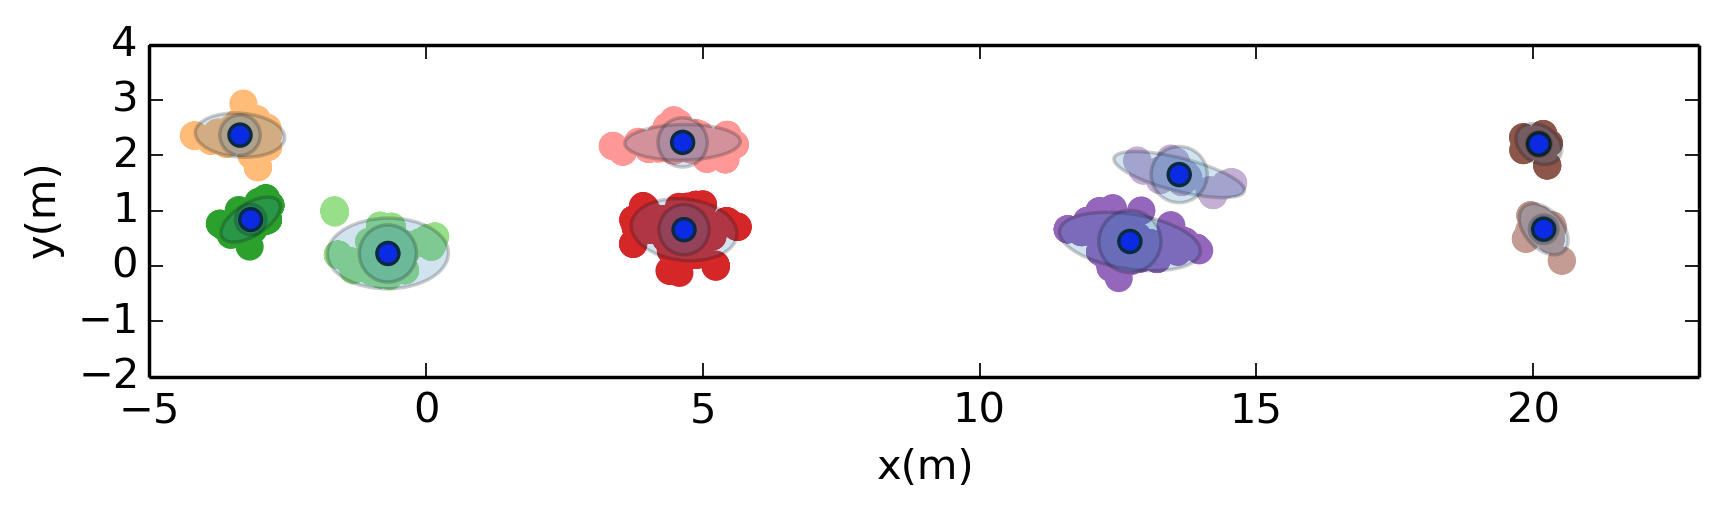
\includegraphics[]{../savedData/pillar00-new.png}

\begin{tabular}{r|llll}
	\toprule%
	\bfseries Pillar & \bfseries Hits & \bfseries RMS(m) & \bfseries Ellipse x(m) & \bfseries Ellipse y(m)\\\midrule\\[-0.8cm]
	\csvreader[%
	  no head,
	  before line=\ifthenelse{\equal{\csvcoli}{Average}}{\\\midrule}{\\},
	  late after last line = \\\bottomrule,
	]{../savedData/pillar00-new-rounded.csv}{}{%
	  \csvcoli&\csvcolii&\csvcoliii&\csvcoliv&\csvcolv
	}
\end{tabular}
\end{center}



\newpage
\section{Radius 10 cm}
\begin{center}

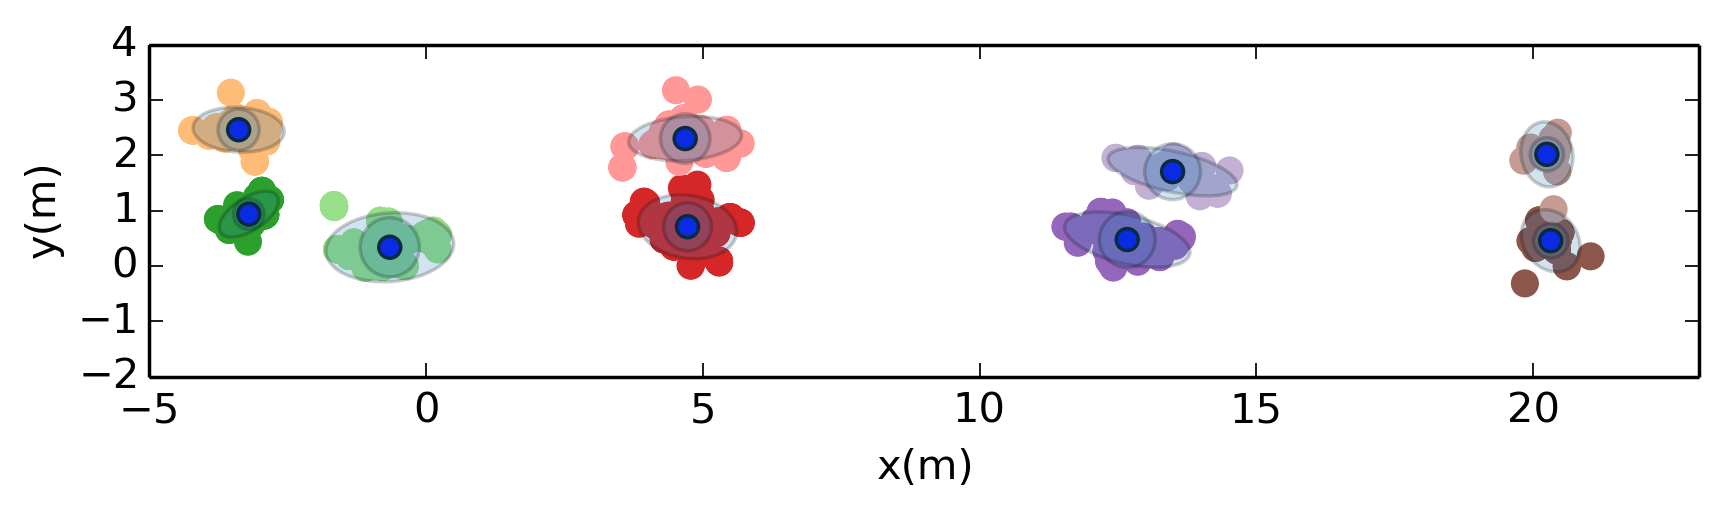
\includegraphics[]{../savedData/pillar01-new.png}

\begin{tabular}{r|llll}
	\toprule%
	\bfseries Pillar & \bfseries Hits & \bfseries RMS(m) & \bfseries Ellipse x(m) & \bfseries Ellipse y(m)\\\midrule\\[-0.8cm]
	\csvreader[%
	  no head,
	  before line=\ifthenelse{\equal{\csvcoli}{Average}}{\\\midrule}{\\},
	  late after last line = \\\bottomrule,
	]{../savedData/pillar01-new-rounded.csv}{}{%
	  \csvcoli&\csvcolii&\csvcoliii&\csvcoliv&\csvcolv
	}
\end{tabular}
\end{center}


\section{Radius 20 cm}
\begin{center}
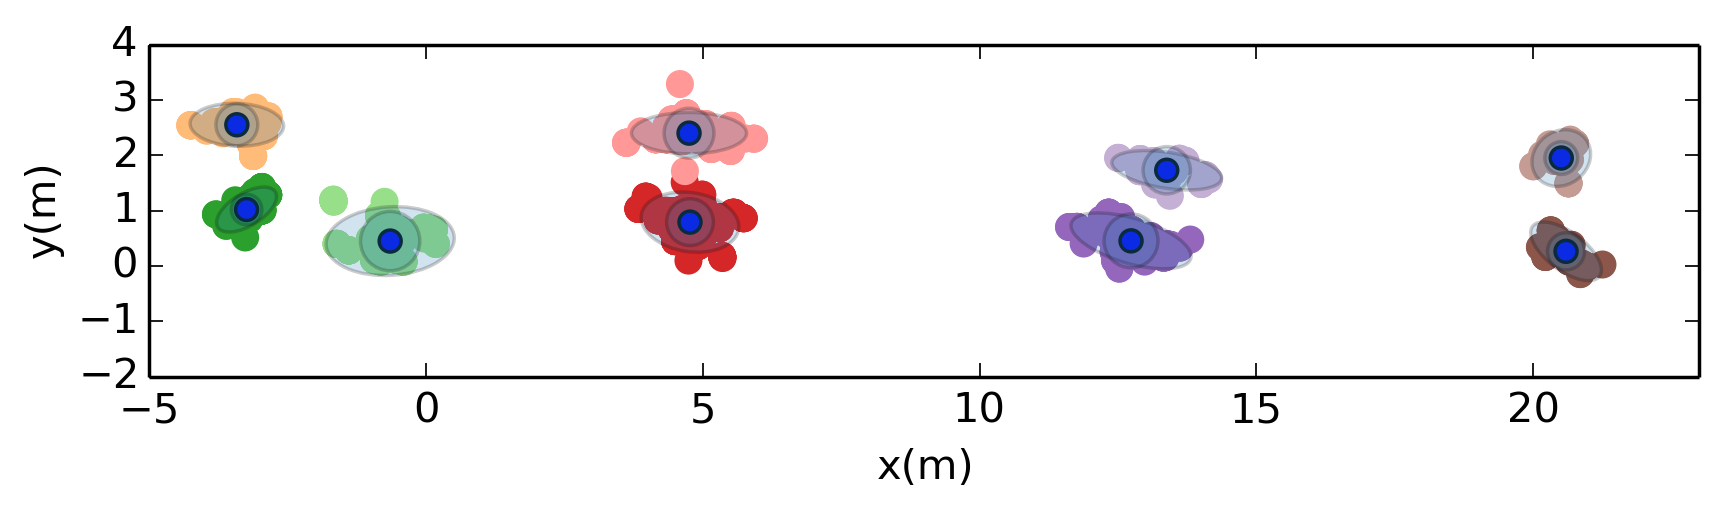
\includegraphics[]{../savedData/pillar02-new.png}

\begin{tabular}{r|llll}
	\toprule%
	\bfseries Pillar & \bfseries Hits & \bfseries RMS(m) & \bfseries Ellipse x(m) & \bfseries Ellipse y(m)\\\midrule\\[-0.8cm]
	\csvreader[%
	  no head,
	  before line=\ifthenelse{\equal{\csvcoli}{Average}}{\\\midrule}{\\},
	  late after last line = \\\bottomrule,
	]{../savedData/pillar02-new-rounded.csv}{}{%
	  \csvcoli&\csvcolii&\csvcoliii&\csvcoliv&\csvcolv
	}
\end{tabular}
\end{center}

\newpage


\section{Radius 30 cm}
\begin{center}
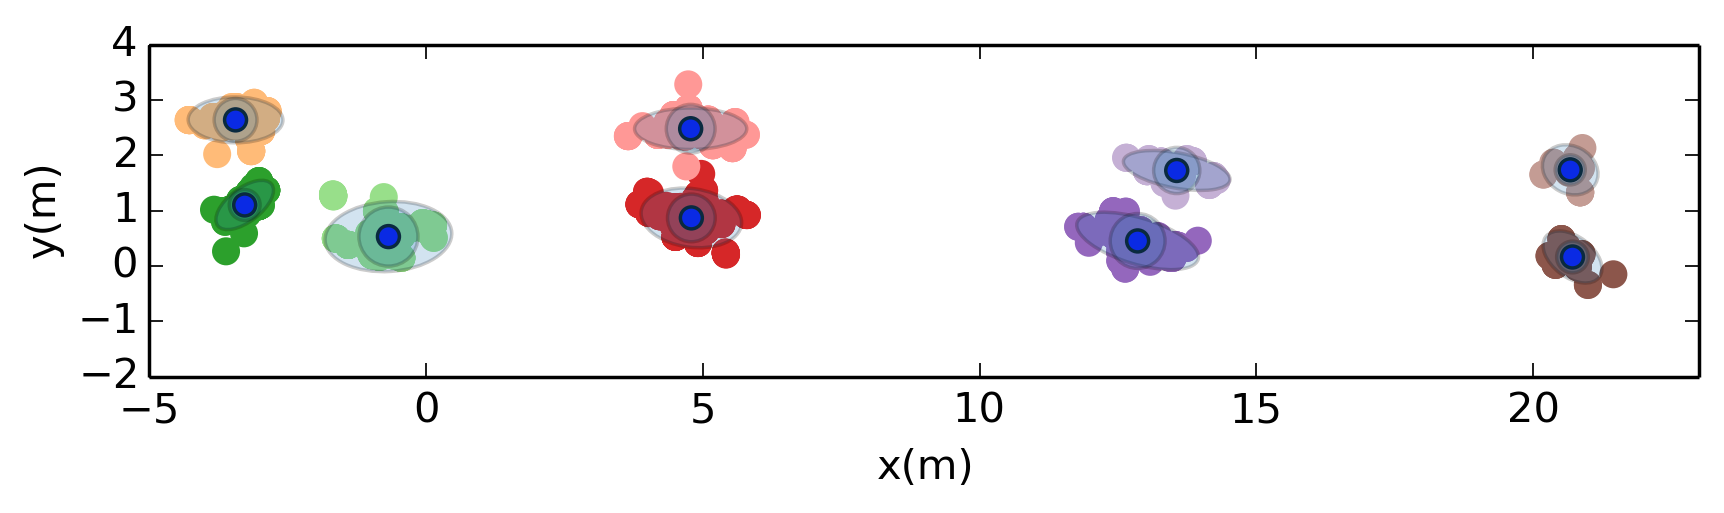
\includegraphics[]{../savedData/pillar03-new.png}

\begin{tabular}{r|llll}
	\toprule%
	\bfseries Pillar & \bfseries Hits & \bfseries RMS(m) & \bfseries Ellipse x(m) & \bfseries Ellipse y(m)\\\midrule\\[-0.8cm]
	\csvreader[%
	  no head,
	  before line=\ifthenelse{\equal{\csvcoli}{Average}}{\\\midrule}{\\},
	  late after last line = \\\bottomrule,
	]{../savedData/pillar03-new-rounded.csv}{}{%
	  \csvcoli&\csvcolii&\csvcoliii&\csvcoliv&\csvcolv
	}
\end{tabular}
\end{center}



\section{Radius 40 cm}
\begin{center}
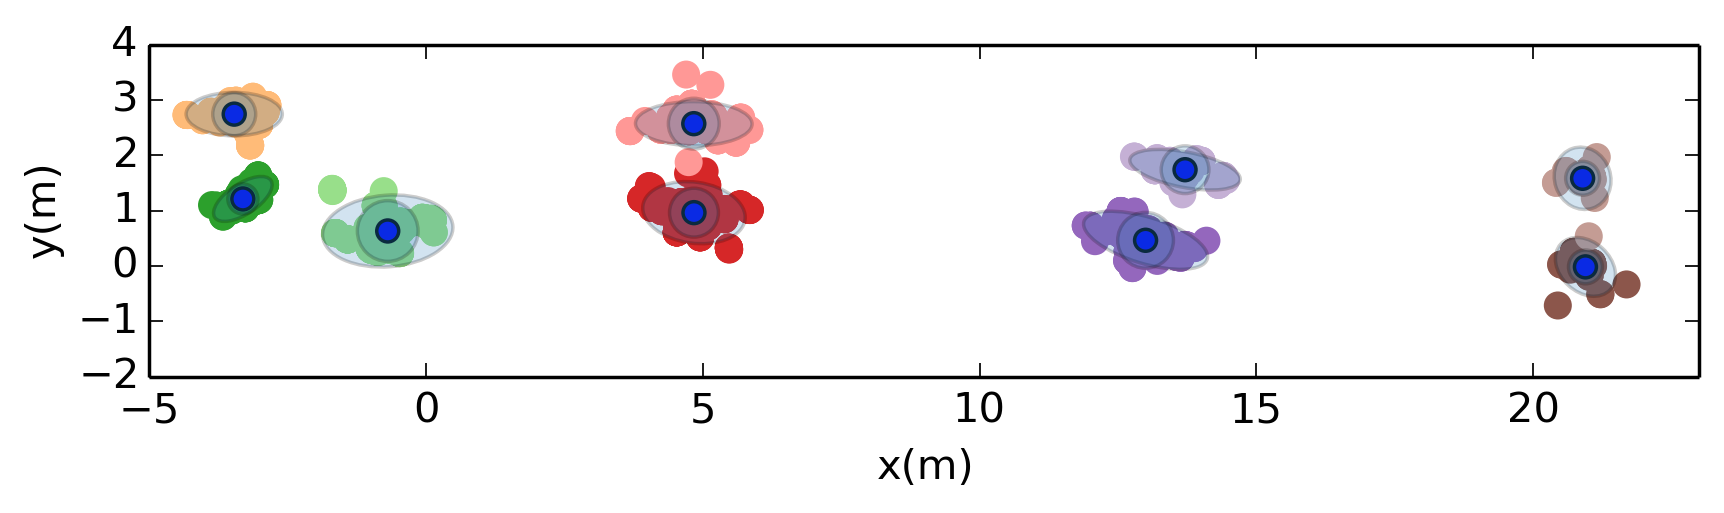
\includegraphics[]{../savedData/pillar04-new.png}

\begin{tabular}{r|llll}
	\toprule%
	\bfseries Pillar & \bfseries Hits & \bfseries RMS(m) & \bfseries Ellipse x(m) & \bfseries Ellipse y(m)\\\midrule\\[-0.8cm]
	\csvreader[%
	  no head,
	  before line=\ifthenelse{\equal{\csvcoli}{Average}}{\\\midrule}{\\},
	  late after last line = \\\bottomrule,
	]{../savedData/pillar04-new-rounded.csv}{}{%
	  \csvcoli&\csvcolii&\csvcoliii&\csvcoliv&\csvcolv
	}
\end{tabular}
\end{center}



\newpage

\section{Radius 50 cm}
\begin{center}
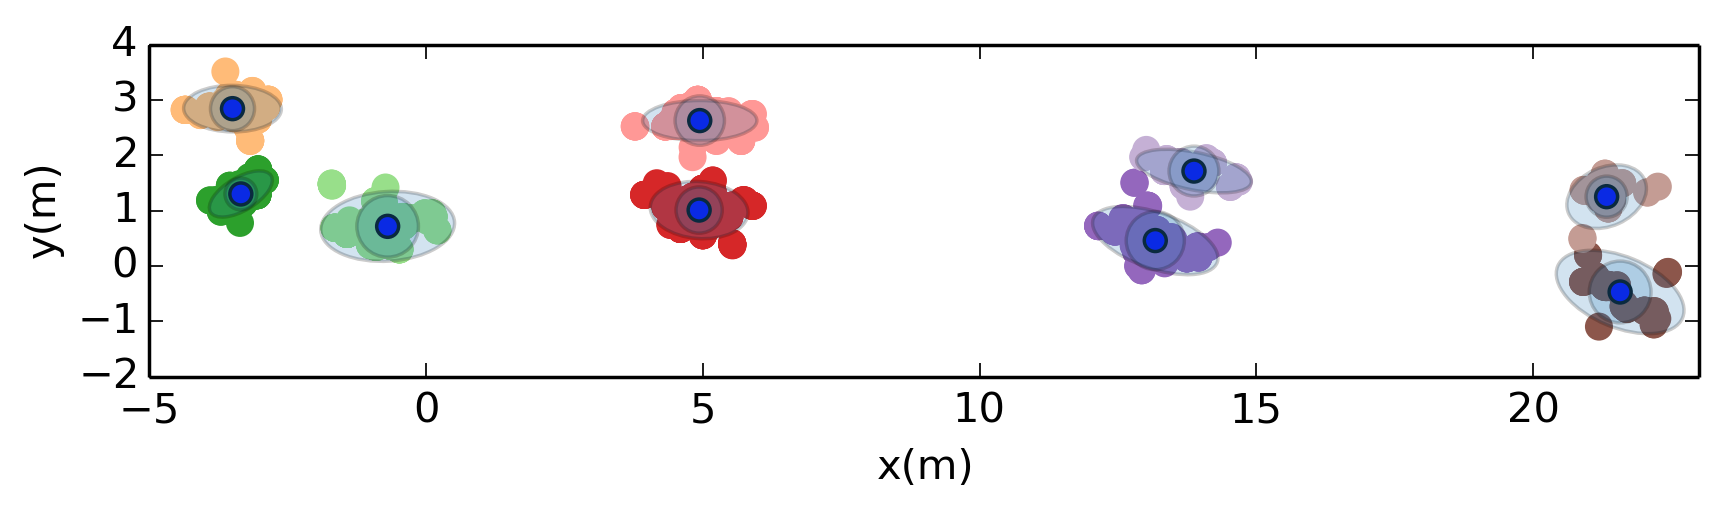
\includegraphics[]{../savedData/pillar05-new.png}

\begin{tabular}{r|llll}
	\toprule%
	\bfseries Pillar & \bfseries Hits & \bfseries RMS(m) & \bfseries Ellipse x(m) & \bfseries Ellipse y(m)\\\midrule\\[-0.8cm]
	\csvreader[%
	  no head,
	  before line=\ifthenelse{\equal{\csvcoli}{Average}}{\\\midrule}{\\},
	  late after last line = \\\bottomrule,
	]{../savedData/pillar05-new-rounded.csv}{}{%
	  \csvcoli&\csvcolii&\csvcoliii&\csvcoliv&\csvcolv
	}
\end{tabular}
\end{center}

\end{document}